\chapter{Wstęp}

	Celem pracy jest wykonanie emulatora procesora Zilog Z80. Aplikacja umożliwia wczytanie programu w postaci kodu maszynowego, deasemblację i wykonanie. Dostępne są dwa tryby wykonania: ciągły i krokowy. W obu przypadkach emulator obrazuje stan rejestrów, jak również umożliwia podgląd i zmianę zawartości pamięci programu. Aplikacja została zaimplementowana w języku Java.
	
	% to jest skopiowane prosto z książki
	Procesor Zilog z80 był szlagierem rynku mikroprocesorowego. \cite{karczmarczuk}
	Został wydany na rynek w roku 1976, i szybko zdominował rynek 8-bitowych procesorów.
	
	Jednym z jego powodów sukcesu na rynku, była prostota w sprzęganiu go z innymi urządzeniami, szczególnie pamięciami. Inną jego zaletą była lista rozkazów zgodna z popularnym w tamtym czasie procesorem, mianowicie Intelem 8086, co umożliwiało uruchamianie programów napisanych z pierwotnym przeznaczeniem dla Intela 8080 na Zilogu Z80. \cite{karczmarczuk}
	
	Urządzenie to mimo zalet, ma również jedną dużą wadę. Jego wewnętrzna budowa była złożona jak na tamte czasy, wyjścia nie były ułożone w logiczny sposób (widoczne na rysunku  \ref{img:z80wyprowadzenia}), a lista rozkazów składała się z 158 pozycji, w tym 78 z nich zgodnych z Intel 8080A \cite{manual}
	
	
	\begin{figure}[h]
		\centering
		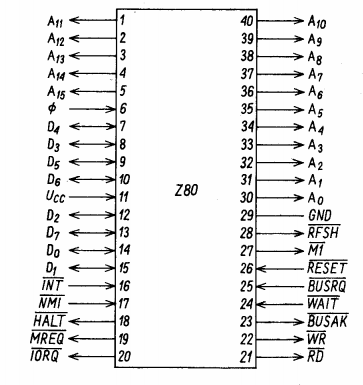
\includegraphics[width=0.5\textwidth]{z80wyprowadzenia}
		\caption{Wyprowadzenia mikroprocesora Z80 \cite{karczmarczuk}}
		\label{img:z80wyprowadzenia}
	\end{figure}
			
	\begin{figure}[h]		
		\centering
		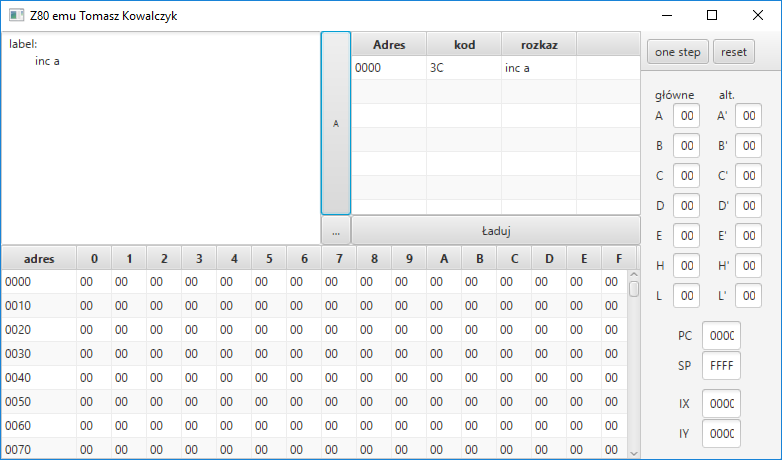
\includegraphics[width=0.6\textwidth]{app1}
		\caption{Widok główny emulatora}
	\end{figure}
	
	Samą aplikacje wykonano w języku Java 8 i biblioteki graficznej Java FX. 
	Interfejs użytkownika został podzielony na 3 części: 
	\begin{itemize}  
		\item widok kodu programu napisany w języku asembler, wraz z  wynikowym kodem maszynowym  
		\item widok pamięci w formie tabeli. Aby uzyskać adres odpowiadający danej komórce, należy dodać do siebie wartość \underline{?????}. Edycje wykonujemy przez dwukrotne kliknięcie w komórkę tabeli, wpisaniu nowej wartości i zatwierdzeniu klawiszem Enter.
		\item widok stanu wewnętrznych rejestrów procesora, wraz z przyciskami debugującymi.   
	\end{itemize}
	
	W aplikacji każda wyświetlona wartość podana jest w systemie heksadecymalnym, i także w takiej notacji wprowadzamy wartości (oprócz pola do edycji kodu asemblera, gdzie możemy używać innych notacji).
	